
\lesson{27/10}
\textbf{Note} The function is named $G$ because it is a \textbf{Green function}
of the operators in the equations of motion of the fields, as will be proven.

\subsection{Naming conventions}
The Feynman propagator is the function $\Delta_F$, which is defined so that
$$i\Delta_f = G(x^\mu,y^\nu);$$
another notation is to indicate the two parts of $G$ as, respectively,
$D(x-y)$, $D(y-x)$:
$$G(x,y) = \vartheta(x^0-y^0)D(x-y) + \vartheta(y^0-x^0)D(y-x).$$
Another important notation is that of the \textit{time ordering operator} $T$:
$$T\psi(x)\chi(y) = \begin{dcases}
    \psi(x)\chi(y) &\text{if }x^0>y^0\\
    \pm\chi(y)\psi(y) &\text{if }y^0>x^0\\
\end{dcases}
$$
where the $+$ is used for scalar fields, while the $-$ for Dirac fields.

This also has a graphical interpretation
\begin{figure}[H]
    \centering
    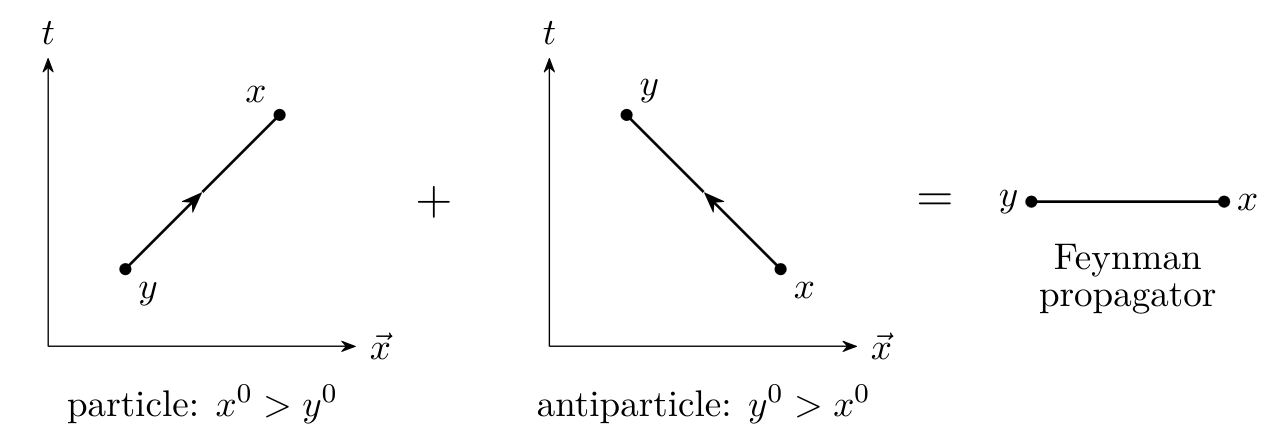
\includegraphics[width = \linewidth]{./F_prop.png}
    \caption{From Prof. Boglione's notes}
\end{figure}
\subsection{Propagator for the scalar field}
The goal is to find the explicit form of the propagator for the
scalar field
$$\phi(x^\mu) = \int \frac{\dd^3p}{(2\pi)^{\flatfrac{3}{2}} \sqrt{2E_p}}\left[
    a_pe^{-ipx}+a^\dagger_pe^{ipx}\right]. $$
Since the field is real, the propagator becomes
$$i\Delta_F = \vartheta(x^0-y^0)\bra{0}\phi(x)\phi(y)\ket{0} +
\vartheta(y^0-x^0)\bra{0}\phi(y)\phi(x)\ket{0}$$
consider
$$\phi(y)\ket{0} = \int \frac{\dd^3p'}{(2\pi)^\frac{3}{2}\sqrt{2E_{p'}}} e^{ip'y}
\ket{\mathbf{p'}}$$
where $a_{p'}\ket{0}=0$ and $a_{p'}^\dagger\ket{0}=\ket{\mathbf{p'}}$. 
Similarly
$$\bra{0}\phi(x)= \int \frac{\dd^3p}{(2\pi)^\frac{3}{2}\sqrt{2E_p}} e^{-ipx}
\bra{\mathbf{p}}$$
and so
$$D(x-y)=\bra{0}\phi(x)\phi(y)\ket{0} = \int \frac{\dd^3p\dd^3p'}{(2\pi)^32
\sqrt{E_pE_{p'}}} e^{-ipx+ip'y}\bra{\mathbf{p}}\ket{\mathbf{p'}} =
\int\frac{\dd^3p}{(2\pi)^32E_p}e^{-ip(x-y)}.$$
Similarly, the second term is
$$D(y-x) = \bra{0}\phi(y)\phi(x)\ket{0} =
\int\frac{\dd^3p}{(2\pi)^32E_p}e^{-ip(y-x)}.$$
and so
$$i\Delta_F = \int \frac{\dd^3p}{(2\pi)^32E_p}\left[\vartheta(x^0-y^0)
    e^{-ip(x-y)} + \vartheta(y^0-x^0)e^{ip(x-y)}
\right]$$
Letting $z^\mu = x^\mu-y^\mu$, the needed functions this is
$$i\Delta_F = \int \frac{\dd^3p}{(2\pi)^32E_p}\left[\vartheta(z^0)
    e^{-ipz} + \vartheta(y^0-x^0)e^{ipz}
\right]$$
To compute the integral explicitely, the theta function integral representation
is needed.
\subsubsection{Integral representation of the theta function}
The Theta function is defined as
$$\vartheta(z^0)=\begin{dcases}
    1&\text{if }z^0\geq0\\
    0&\text{if }z^0\leq0
\end{dcases}.
$$
Consider a complex function with a simple pole in $i\varepsilon$, with
$\varepsilon>0$:
$$\frac{e^{i\tau z_0}}{\tau-i\varepsilon}$$
then its integral over the real axis
$$I(z^0)=\lim\limits_{\varepsilon\to0^+}\frac{1}{2\pi i}\int_{-\infty}^\infty
\dd\tau
\frac{e^{i\tau z^0}}{\tau-i\varepsilon}
$$
can be computed using Jordan's lemma,
depending on the sign of $z^0$: if it is positive the contour is closed in
$\Im(\tau)>0$ and the residue is included in the contour and the integral is
nonzero, while if $z^0$ is negative, the contour must be closed in $\Im(\tau)<0$
and the integral is zero, so
$$I(z^0) = \vartheta(z^0) =\begin{dcases}
    1&\text{if }z^0\geq0\\
    0&\text{if }z^0\leq0
\end{dcases}.
$$\\

Inserting this representation and returning to the full Lorentz-invariant
measure of integration yields
\begin{gather*}
i\Delta_F = \frac{1}{(2\pi)^3}\int d^4p\vartheta(p^0)\delta(p^2-m^2)\left[
\vartheta(z^0) e^{-ipz} + \vartheta(-z^0)e^{ipz}\right]=\\
=\lim\limits_{\varepsilon\to0^+}
\frac{1}{i(2\pi)^4}\int \dd^4p\int_{-\infty}^\infty \dd\tau \vartheta(p^0)
\delta(p^2-m^2)\left\{\frac{e^{-i(pz-\tau z^0)}}{\tau-i\varepsilon}
+ \frac{e^{i(pz-\tau z^0)}}{\tau-i\varepsilon}\right\}
\end{gather*}
The strategy here is to find a new variable so that the second exponential
has the same sign as the first.
Letting
$$p'^0 = p^0-\tau,\;\mathbf{p'=p},\;\omega_{p'}^2:=\mathbf{p'}^2+m^2\implies
\omega_{p'}^2-(p'^0)^2 = m^2 - (p')^2$$
modifies the mass-shell:
$$\delta(p^2-m^2)=\delta((p'^0+\tau)^2-\omega_{p'}^2) = \frac{\delta(p'^0+\tau+
\omega_{p'})}{2\omega_{p'}} + \frac{\delta(p'^0+\tau-\omega_{p'})}{2\omega_{p'}}$$
[something with the product with $\vartheta(p^0)$]
$$i\Delta_F = \frac{1}{i(2\pi)^4}\int \dd^4p'\int_{-\infty}^\infty \dd\tau
e^{-ip'z}\left\{\frac{\delta(p'^0+\tau+\omega_{p'})}{2\omega_{p'}} +
\frac{\delta(p'^0+\tau-\omega_{p'})}{2\omega_{p'}}\right\}\left\{
\frac{\vartheta(p'^0+\tau)}{\tau-i\varepsilon}+\frac{\vartheta(p'^0-\tau)}
{\tau-i\varepsilon}\right\}
$$
2 out of the 4 products contain incompatible products of $\delta$ and $\vartheta$\\
\{vedi foto per il continuo dei conti + note boglione\}
\\
The final result is
$$\boxed{\Delta_F(x-y) = \lim\limits_{\varepsilon\to0^+}\frac{1}{(2\pi)^4}
\int \dd^4p \frac{e^{-ip(x-y)}}{p^2-m^2+i\varepsilon}}$$
Its Fourier transform in the momentum space is manifest
$$\Delta_F(p) = \lim\limits_{\varepsilon\to0^+}\frac{1}{p^2-m^2+i\varepsilon}$$
\textbf{Note} The $i\varepsilon$ at the denominators come from the $\vartheta$, so
they guarantee causality.
